%------------------------------------------------------------------------
%Editar Diplomado
\hypertarget{cv:GestionarCU}{\section{Gestionar Casos de Uso}} \label{sec:GestionarCU}

	Esta funcionalidad le permitirá las acciones necesarias para controlar los casos de uso y visualizarlos en una tabla en el proyecto sobre el que se está operando y solicitar el registro de uno nuevo.

		\subsection{Procedimiento}

			%Pasos de procedimiento
			\begin{enumerate}
				
			\item Ingrese a un proyecto existente desde la pantalla \ref{fig:GestionarProyectosColaborador}.
			
			\item Oprima el botón \IUCU{} de algún registro existente de la pantalla \ref{fig:GestionarModulos} ''Gestionar Módulos''.
	
			\item Se mostrará la pantalla \ref{fig:GestionarCU} ''Gestionar Casos de Uso''.

			%Pantalla
			\begin{figure}[htbp!]
				\begin{center}
					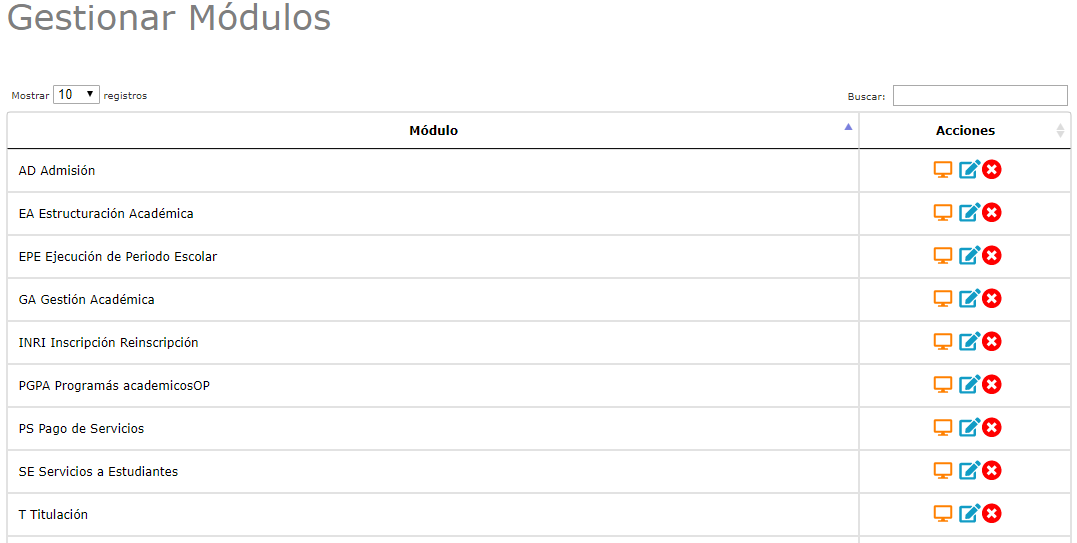
\includegraphics[scale=0.6]{roles/lider/casosUso/pantallas/IU5gestionarModulos}
					\caption{Gestionar Casos de Uso}
					\label{fig:GestionarCU}
				\end{center}
			\end{figure}
		
				\item Seleccione la operación que desea realizar:
			
			Para (\hyperlink{cv:registrarCU}{Registrar}) dé clic en el botón \IURegistrar.
			
			Para (\hyperlink{cv:modificarCU}{Modificar}) dé clic en el icono \IUEditar{} de algún caso de uso ya registrado.
			
			Para (\hyperlink{cv:eliminarCU}{Eliminar}) dé clic en el icono \IUBotonEliminar{} de algún caso de uso ya registrado.
			
			Para (\hyperlink{cv:consultarCU}{Consultar}) dé clic en el icono \IUConsultar{} de algún caso de uso ya registrado.
			
			Para (\hyperlink{cv:terminarCU}{Terminar Caso de uso}) dé clic en el icono \IUTerminar{} de algún caso de uso ya registrado.
			
			Para (\hyperlink{cv:revisarCU}{Revisar Caso de uso}) dé clic en el icono \IURevisar{} de algún caso de uso ya registrado.
			
			Para (\hyperlink{cv:GestionarTray}{Gestionar Trayectorias}) dé clic en el icono \IUTray{} de algún caso de uso ya registrado.
			
			Para (\hyperlink{cv:GestionarPrecondiciones}{Gestionar Precondiciones}) dé clic en el icono PENDIENTE de algún caso de uso ya registrado.
			
			Para (\hyperlink{cv:GestionarTray}{Gestionar Postcondiciones}) dé clic en el icono PENDIENTE de algún caso de uso ya registrado.
			\end{enumerate}